\chapter{车道汇合群决策模型仿真}
% 仿真的一些综述

\section{仿真平台设计}
为了实现对上述控制算法的仿真,本课题中使用{\ttfamily Python}开发仿真程序。仿真程序大体框架如图\ref{fig:ss}。
\subsection{仿真程序结构}
\begin{figure}
\centering
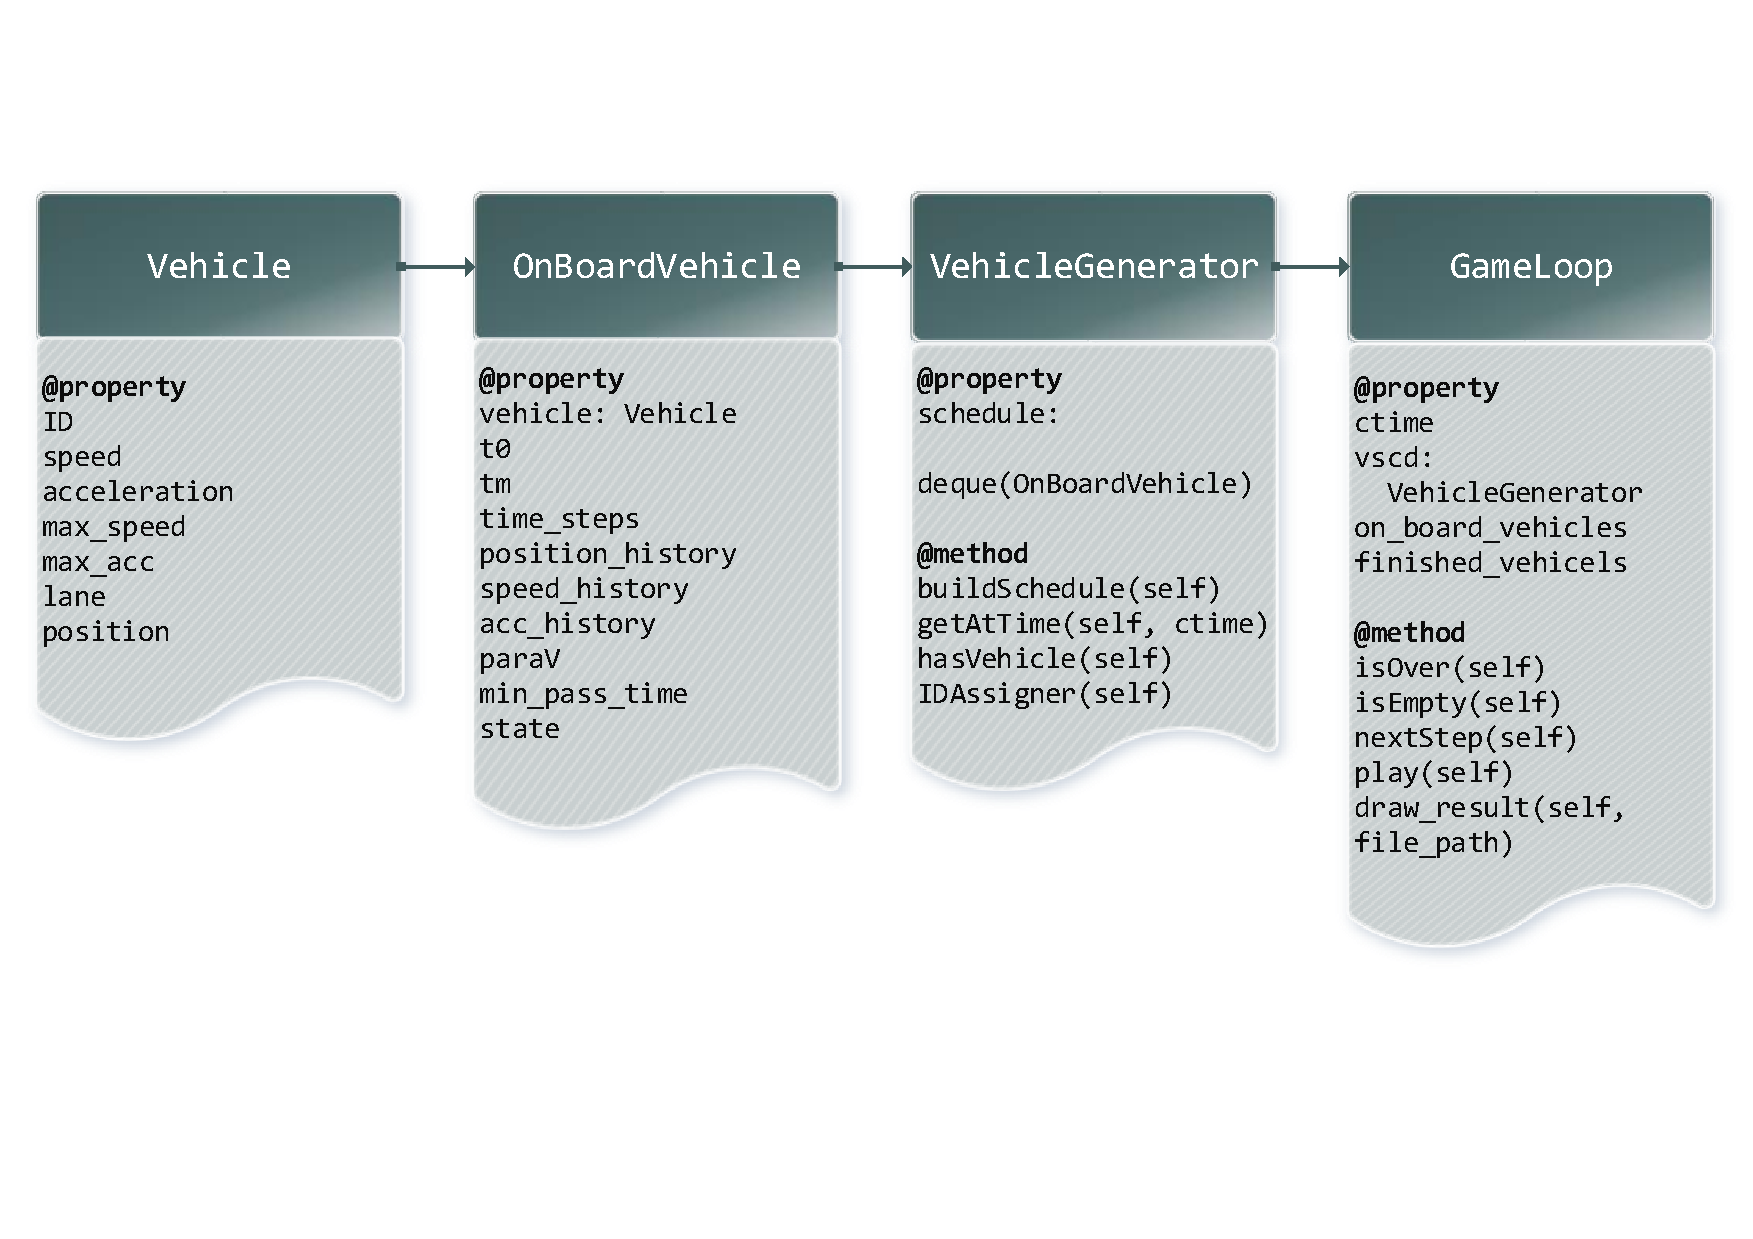
\includegraphics[width=15cm,trim={0 4cm 0 2cm},clip]{figures/software_structure.pdf}
\caption{仿真程序结构}
\label{fig:ss}
\end{figure}
\subsection{网页仿真平台设计}


\section{简单FIFO序列仿真}
\subsection{相同速度进入控制区}
下面考虑最简单的情况,同一车道上的车辆按照相同速度进入控制区。其中主路进入速度
仿真结果如图\ref{fig:case1:posi}---\ref{fig:case1:fuel}
\begin{figure}
\begin{minipage}{0.48\textwidth}
  \centering
  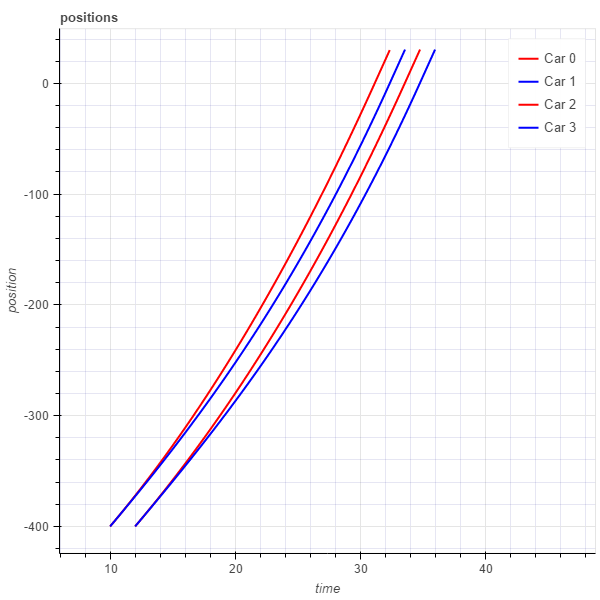
\includegraphics[height=6cm]{figures/sim_case1/posi.png}
  \caption{位移-时间关系图(第一组)}
  \label{fig:case1:posi}
\end{minipage}\hfill
\begin{minipage}{0.48\textwidth}
  \centering
  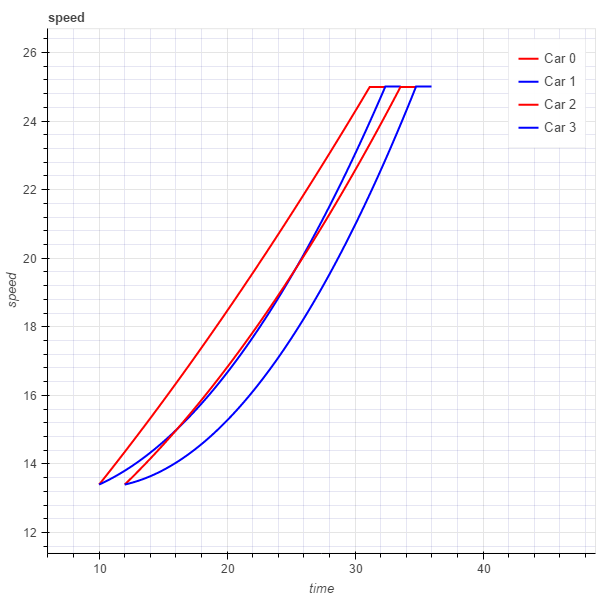
\includegraphics[height=6cm]{figures/sim_case1/speed.png}
  \caption{速度-时间关系图(第一组)}
  \label{fig:case1:speed}
\end{minipage}
\end{figure}
\begin{figure}
\begin{minipage}{0.48\textwidth}
  \centering
  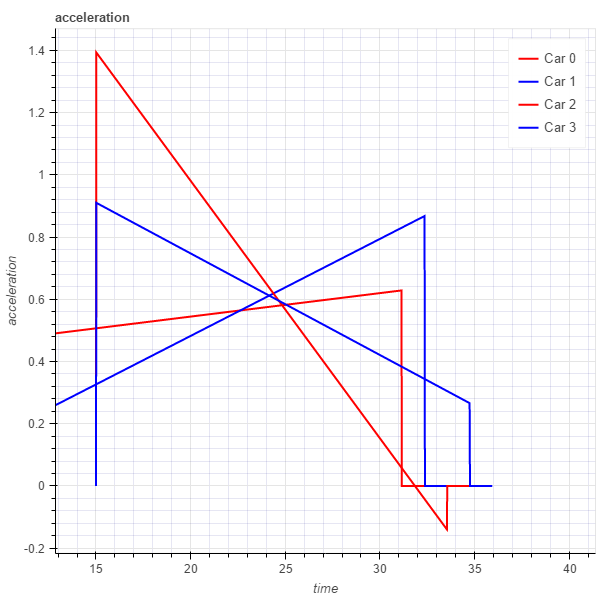
\includegraphics[height=6cm]{figures/sim_case1/acc.png}
  \caption{加速度-时间关系图(第一组)}
  \label{fig:case1:acc}
\end{minipage}\hfill
\begin{minipage}{0.48\textwidth}
  \centering
  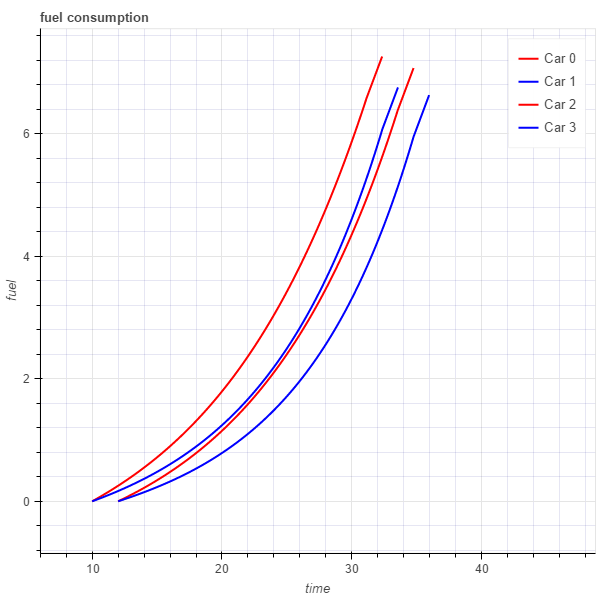
\includegraphics[height=6cm]{figures/sim_case1/fuel.png}
  \caption{油耗-时间关系图(第一组)}
  \label{fig:case1:fuel}
\end{minipage}
\end{figure}

\subsection{主辅路不同速度进入控制区}
\subsection{随机速度进入控制区}

\section{改进的优先到达序列仿真}
\subsection{排序原理}
\subsection{时间目标优先}
\subsection{系统能量目标优先}

\chapter{群决策模型改进}
(有时候由于信息不准或延迟,可能控制区会撞)
\section{碰撞紧急修正处理}
\subsection{修正必要性与原理}
\subsection{带有修正的系统仿真}
\section{}

\chapter{总结与展望}